\documentclass[11pt,preprint]{elsarticle}
\usepackage[latin9]{inputenc}
\usepackage{geometry}
\geometry{verbose,tmargin=1cm,bmargin=1cm,lmargin=1cm,rmargin=1cm,headheight=1cm,headsep=1cm,footskip=2cm}
\usepackage{float}
\usepackage{amsmath}
\usepackage{amssymb}
\usepackage{graphicx}
\usepackage{esint}

\makeatletter

\newcounter{bla}
\newenvironment{refnummer}{%
\list{[\arabic{bla}]}%
{\usecounter{bla}%
 \setlength{\itemindent}{0pt}%
 \setlength{\topsep}{0pt}%
 \setlength{\itemsep}{0pt}%
 \setlength{\labelsep}{2pt}%
 \setlength{\listparindent}{0pt}%
 \settowidth{\labelwidth}{[9]}%
 \setlength{\leftmargin}{\labelwidth}%
 \addtolength{\leftmargin}{\labelsep}%
 \setlength{\rightmargin}{0pt}}}{\endlist}

\journal{Computer Physics Communications}

% Paquets
\usepackage{multicol}

\makeatother

\begin{document}
\begin{frontmatter}



\title{Collision operator of GYSELA}


\author{P. Donnel}


%% Text of abstract
\begin{abstract}
The collision operator used in GYSELA is described in this note. For more details please read the associated paper \cite{Donnel_CPC_2019}
\end{abstract}

\end{frontmatter}


\section{Presentation of the model}

The linearized collisional operator describing the collisions of species
$a$ colliding on species $b$ takes the form
\[
C_{ab}(F_{a},F_{b})=C_{ab}^{0}(F_{M0a},F_{M0b})+C_{ab}^{1}(F_{a},F_{b}) ,
\]
where $F_{M0a}$ represents the local unshifted Maxwellian with density
$n_{a}$ and temperature $T_{a}$

\[
F_{M0a}(\boldsymbol{x},\boldsymbol{v},t)=n_{a}(\boldsymbol{x},t)\left(\frac{1}{2\pi v_{Ta}^{\text{2}}}\right)^{3/2}\exp\left(-x_{a}^{2}\right) .
\]
A normalized speed has been used $x_{a}=\frac{v}{\sqrt{2}v_{Ta}}$
,with $v_{Ta}=\sqrt{\frac{T_{a}}{m_{a}}}$ the thermal velocity. 

$C_{ab}^{0}$ represents the exchange of energy between the unshifted
Maxwellians
\[
C_{ab}^{0}(F_{M0a},F_{M0b})=\frac{T_{b}-T_{a}}{T_{b}}x_{a}^{2}\nu_{E,ab}F_{M0a}
\]


Neglecting all finite Larmor radius effects, $C_{ab}^{1}$ is composed
of three terms 
\[
C_{ab}^{1}(F_{a},F_{b})=C_{v,ab}(F_{a})+C_{d,ab}(F_{a})+C_{\parallel,ab}(F_{a},F_{b})
\]


$C_{v,ab}$ is an operator acting on the norm of the velocity. When
written in the set of variables $\left(v_{\parallel},v_{\perp}\right)$,
it reads as follows:

\begin{eqnarray*}
C_{v,ab}\left(F_{a}\right) & = & \frac{1}{2v_{\perp}}\frac{\partial}{\partial v_{\perp}}\left[F_{M0a}\nu_{v,ab}v_{\perp}^{2}\left(v_{\perp}\frac{\partial g_{ab}}{\partial v_{\perp}}+v_{\parallel}\frac{\partial g_{ab}}{\partial v_{\parallel}}\right)\right]\\
 & + & \frac{1}{2}\frac{\partial}{\partial v_{\parallel}}\left[F_{M0a}\nu_{v,ab}v_{\parallel}\left(v_{\perp}\frac{\partial g_{ab}}{\partial v_{\perp}}+v_{\parallel}\frac{\partial g_{ab}}{\partial v_{\parallel}}\right)\right]
\end{eqnarray*}


$C_{d,ab}$ modifies the direction of the velocity vector
(deflection)
\begin{eqnarray*}
C_{d,ab}\left(F_{a}\right) & = & \frac{1}{2v_{\perp}}\frac{\partial}{\partial v_{\perp}}\left[F_{M0a}\nu_{d,ab}v_{\perp}v_{\parallel}\left(v_{\parallel}\frac{\partial g_{ab}}{\partial v_{\perp}}-v_{\perp}\frac{\partial g_{ab}}{\partial v_{\parallel}}\right)\right]\\
 & + & \frac{1}{2}\frac{\partial}{\partial v_{\parallel}}\left[F_{M0a}\nu_{d,ab}v_{\perp}\left(-v_{\parallel}\frac{\partial g_{ab}}{\partial v_{\perp}}+v_{\perp}\frac{\partial g_{ab}}{\partial v_{\parallel}}\right)\right]
\end{eqnarray*}


Finally the term $C_{\parallel,ab}$ ensures momentum exchange between
species and the conservation of the total parallel momentum.

\[
C_{\parallel,ab}\left(F_{a},F_{b}\right)=-\frac{\nu_{s,ab}(v)}{v_{Ta}^{2}}v_{\parallel}\left(U_{\parallel d,a}-U_{\parallel ba}\right)F_{M0a}
\]


The normalized distribution function has to be shifted to ensure that
$C_{v,ab}$ and $C_{d,ab}$ conserve momentum and energy 
\[
g_{ab}=f_{a}-\frac{v_{\parallel}U_{\parallel d,a}}{v_{Ta}^{2}}-x_{a}^{2}q_{ba}\text{ with }\ensuremath{f_{a}=\frac{F_{a}}{F_{M0a}}}
\]


More specifically, $U_{\parallel d,a}$ ensures that $C_{v,ab}$ and
$C_{d,ab}$ conserve momentum.

\[
\frac{v}{v_{Ta}^{2}}U_{\parallel d,a}\left(v\right)=\frac{3}{2}\int d\xi\xi f_{a}\text{ with \ensuremath{\xi=\frac{v_{\parallel}}{v}} }
\]


Then in order to take into account momentum exchange between species
while keeping the total momentum constant, a second velocity $U_{\parallel ab}$
is chosen as
\[
U_{\parallel ab}=\frac{\left\langle \nu_{s,ab}v^{2}U_{\parallel d,a}\right\rangle _{a}}{\left\langle \nu_{s,ab}v^{2}\right\rangle _{a}}
\]


A dimensionless parameter $q_{ab}$ accounting for energy exchange
between species is defined as
\[
q_{ab}=T_{b}\frac{\left\langle \nu_{E,ab}\frac{m_{a}v^{2}}{2}f_{a}\right\rangle _{a}}{\left\langle \nu_{E,ab}\left(\frac{m_{a}v^{2}}{2}\right)^{2}\right\rangle _{a}}
\]


The bracket corresponds to mean values in velocity space $<...>=\int d^{3}\boldsymbol{v}\frac{F_{M0a}}{n_{a}}...$
. Different frequencies appear in the previous expressions. They are
defined as follow :
\begin{itemize}
\item the Hirshman and Sigmar's inter-species collision frequency 
\end{itemize}
\[
\nu_{ab}^{HS}=\sqrt{2}\frac{N_{b}Z_{b}^{2}}{N_{a}Z_{a}^{2}}\nu_{aa}
\]

\begin{itemize}
\item the velocity modulus diffusion rate 
\end{itemize}
\[
\nu_{v,ab}\left(x_{a}\right)=\nu_{ab}^{HS}x_{ba}\frac{\Theta\left(x_{b}\right)}{x_{a}^{2}}
\]

\begin{itemize}
\item the deflection frequency 
\end{itemize}
\[
\nu_{d,ab}\left(x_{a}\right)=\nu_{ab}^{HS}x_{ba}\frac{\Psi\left(x_{b}\right)}{x_{a}^{2}}
\]

\begin{itemize}
\item the slowing-down frequency
\end{itemize}
\[
\nu_{s,ab}=\nu_{ab}^{HS}\left(1+\frac{m_{a}}{m_{b}}\right)x_{ba}^{3}\Theta(x_{b})
\]

\begin{itemize}
\item the energy-loss rate is defined as
\end{itemize}
\[
\nu_{E,ab}=-\frac{1}{v^{4}F_{M0a}}\frac{\partial}{\partial v}\left(\nu_{v,ab}F_{M0a}v^{5}\right)
\]


Where the ratio between the thermal velocities is introduced $x_{ba}=\frac{v_{Ta}}{v_{Tb}}$.
We also define the following functions
\[
\Psi\left(x\right)=\frac{3\sqrt{\pi}}{4}\frac{1}{x}\left[\Phi\left(x\right)-G\left(x\right)\right]
\]
\[
\Theta\left(x\right)=\frac{3\sqrt{\pi}}{2}\frac{G\left(x\right)}{x}
\]


\[
G\left(x\right)=\frac{1}{2x^{2}}\left[\Phi\left(x\right)-x\Phi^{'}\left(x\right)\right]
\]
\[
\Phi\left(x\right)=\frac{2}{\sqrt{\pi}}\int_{0}^{x}dy\exp\left(-y^{2}\right)
\]


The function $\Phi$ is the error function and $G$ is the Chandrasekhar
function. 

\section{Numerical implementation of the collision operator}


\subsection{Separation of the different collision terms}

The collision operator is difficult to treat as a whole. It is much easier to split the different parts of the operator and treat them separately with a time splitting scheme. The time splitting is the following:

\begin{equation}
\begin{cases}
\frac{\partial F_{M0a}}{\partial t}=\sum_{b}C_{ab}^{0}\left(F_{M0a},F_{M0b}\right) & (\Delta t / 2)\\
\frac{\partial F_{a}}{\partial t}=\sum_{b}C_{\parallel,ab}\left(F_{a},F_{b}\right) & (\Delta t / 2)\\
\frac{\partial F_{a}}{\partial t}=\sum_{b}C_{v,ab}\left(F_{a},F_{b}\right)+C_{d,ab}\left(F_{a},F_{b}\right) & (\Delta t) \\
\frac{\partial F_{a}}{\partial t}=\sum_{b}C_{\parallel,ab}\left(F_{a},F_{b}\right) & (\Delta t / 2)\\
\frac{\partial F_{M0a}}{\partial t}=\sum_{b}C_{ab}^{0}\left(F_{M0a},F_{M0b}\right) & (\Delta t / 2)
\end{cases}\label{eq:system of equation to solve}
\end{equation}

In the following, we describe the three

\subsection{Evolution due to $C_{ab}^{0}$ }

The term 
\begin{equation*}
    \frac{\partial F_{M0a}}{\partial t}=\sum_{b}C_{ab}^{0}\left(F_{M0a},F_{M0b}\right)
\end{equation*}
is equivalent to
\begin{equation}
\frac{\partial T_{a}}{\partial t}=\sum_{b}m_{a}\nu_{ab}\left[\frac{2}{m_{a}+m_{b}}\left(T_{b}-T_{a}\right)+\frac{2}{3}V_{\parallel a}\left(V_{\parallel a}-V_{\parallel b}\right)\right]\label{eq:evolution_Maxwellian}
\end{equation}

\subsection{Evolution due to $C_{\parallel,ab}$ }



\begin{eqnarray}
C_{\parallel,ab} & = & \nu_{s,ab}\frac{m_{a}}{T_{a}}v_{\parallel}F_{M0a}\\
 & \times & \left[V_{\parallel b}-V_{\parallel a}+\frac{q_{\parallel a}}{n_{a}T_{a}}\left(1-\frac{2}{5}x_{a}^{2}\right)-\frac{3}{5}\frac{q_{\parallel b}}{n_{b}T_{b}}\left(\frac{1}{1+x_{ba}^{2}}\right)\right] \nonumber
\end{eqnarray}

\subsection{Evolution due to $C_{v,ab}+C_{d,ab}$ }


This is by far the most difficult part of the collision operator. We use the fact that

\begin{equation}
\frac{\partial F_{a}}{\partial t}=\sum_{b}C_{v,ab}\left(F_{a},F_{b}\right)+C_{d,ab}\left(F_{a},F_{b}\right)\Leftrightarrow\frac{\partial f_{a}}{\partial t}=\sum_{b}\bar{C}{}_{ab}\label{eq:equation=0000E0resoudre}
\end{equation}
where we have defined the normalized collision operator $\bar{C}_{ab}(F)=\frac{C_{v,ab}(F)+C_{d,ab}(F)}{F_{M0a}}$.
This approach is possible because a Maxwellian is in the kernel of $C_{v,ab}+C_{d,ab}$. 

The derivatives with respect to $v_{\perp}$ are treated by projecting the distribution in this direction on an orthogonal basis (Laguerre polynomials), then making evolve the projection coefficients and finally coming back on the distribution function. The reason for this choice is the relatively low number of grid points in this direction (typically between 32 and 64).
The first step is therefore to compute the projection of the normalized distribution function

\[
f_{a}(\boldsymbol{r},v_{\parallel},u,t)=\sum_{l}\alpha_{\ell,a}(\boldsymbol{\boldsymbol{r}},v_{\parallel},t)P_{\ell}(u)
\]
where Laguerre polynomials are chosen. The associated scalar product is
\[
\left\langle f|g\right\rangle =\int_{0}^{\infty}dxe^{-x}f\left(x\right)g\left(x\right)
\]
Therefore one has
\[
\alpha_{\ell,a}(\boldsymbol{\boldsymbol{r}},v_{\parallel},t) = \left\langle f_{a}|P_{\ell}\right\rangle =\int_{0}^{\infty}due^{-u}f_{a}\left(u\right)P_{\ell}\left(u\right)
\]
where $u = \frac{\mu B}{T}$

We then define
\[
\begin{cases}
\alpha'_{i,a}=\alpha_{i,a}+\kappa_{i,a} & \text{if \ensuremath{i<2}}\\
\alpha'_{i,a}=\alpha_{i,a} & \text{otherwise}
\end{cases}
\]
with 
\[
\kappa_{0,a}=-\left\{ \frac{m_{a}v_{\parallel}}{T_{a}}\left[V_{\parallel a}-\frac{q_{\parallel a}}{n_{a}T_{a}}\left(\frac{3}{5}-\frac{m_{a}v_{\parallel}^{2}}{5T_{a}}\right)\right]\right\} 
\]
and
\[
\kappa_{1,a}=\frac{2m_{a}v_{\parallel}q_{\parallel a}}{5n_{a}T_{a}^{2}}
\]

The evolution of the coefficients is given by

\begin{equation}
\frac{\partial\alpha_{\ell,a}}{\partial t}=\sum_{j}\left[\alpha_{j,a}^{'}N_{0,a}^{jl}+\frac{\partial\alpha_{j,a}^{'}}{\partial v_{\parallel}}N_{1,a}^{jl}+\frac{\partial^{2}\alpha_{j,a}^{'}}{\partial v_{\parallel}^{2}}N_{2,a}^{jl}\right]\label{eq:projection detaillee}
\end{equation}
with
\begin{eqnarray*}
N_{0,a}^{jl} & = & j\sum_{b}\sum_{i=0}^{j+\ell}C_{j\ell}^{i}\left[\begin{array}{c}
-2L_{i,ab}^{(0)}+2L_{i,ab}^{(1)}+\left(3-\frac{v_{\parallel}^{2}}{v_{Ta}^{2}}\right)L_{i,ab}^{(2)}\\
-2L_{i+1,ab}^{(2)}+\left(2+\frac{v_{\parallel}^{2}}{v_{Ta}^{2}}\right)L_{i,ab}^{(4)}
\end{array}\right]\\
 & - & j\sum_{b}\sum_{i'=0}^{j+\ell-1}C_{j-1,\ell}^{i'}\left[\begin{array}{c}
2L_{i',ab}^{(1)}+\left(3-\frac{v_{\parallel}^{2}}{v_{Ta}^{2}}\right)L_{i',ab}^{(2)}\\
+\left(2+\frac{v_{\parallel}^{2}}{v_{Ta}^{2}}\right)L_{i',ab}^{(4)}
\end{array}\right]
\end{eqnarray*}
\begin{eqnarray*}
N_{1,a}^{jl} & = & v_{\parallel}\sum_{b}\sum_{i=0}^{j+\ell}C_{j\ell}^{i}\left[\begin{array}{c}
-L_{i,ab}^{(0)}+L_{i,ab}^{(1)}+\left(2+2j-\frac{v_{\parallel}^{2}}{2v_{Ta}^{2}}\right)L_{i,ab}^{(2)}\\
-L_{i+1,ab}^{(2)}+L_{i,ab}^{(3)}
\end{array}\right]\\
 & - & v_{\parallel}\sum_{b}\sum_{i'=0}^{j+\ell-1}C_{j-1,\ell}^{i'}2jL_{i',ab}^{(2)}
\end{eqnarray*}
\[
N_{2,a}^{jl}=\sum_{b}\sum_{i=0}^{j+\ell}C_{j\ell}^{i}v_{Ta}^{2}\left[L_{i,ab}^{(0)}+\frac{v_{\parallel}^{2}}{2v_{Ta}^{2}}L_{i,ab}^{(2)}\right]
\]
where the coefficients $C_{j\ell}^{i}$ are defined as
\[
P_{j}\left(u\right) P_{\ell}\left(u\right) = \sum_{i=0}^{j+\ell}C_{j\ell}^{i} u^{i}
\]

It is possible to show that
\[
\begin{cases}
L_{0,ab}^{(1)}= & -\frac{D_{d,ab}\left(v_{\parallel},u=0\right)}{v_{Ta}^{2}}+L_{0,ab}^{(0)}\\
L_{i,ab}^{(1)}= & L_{i,ab}^{(0)}-iL_{i-1,ab}^{(0)}\text{ for \ensuremath{i>0}}
\end{cases}
\]


\[
\begin{cases}
L_{0,ab}^{(3)}= & \frac{v_{\parallel}^{2}}{2v_{Ta}^{2}}\left[L_{0,ab}^{(2)}-\left(\nu_{v,ab}-\nu_{d,ab}\right)\left(v_{\parallel},u=0\right)\right]+L_{1,ab}^{(2)}-L_{0,ab}^{(2)}\\
L_{i,ab}^{(3)}= & \frac{v_{\parallel}^{2}}{2v_{Ta}^{2}}\left[L_{i,ab}^{(2)}-iL_{i-1,ab}^{(2)}\right]+L_{i+1,ab}^{(2)}-\left(i+1\right)L_{i,ab}^{(2)}\text{ for \ensuremath{i>0}}
\end{cases}
\]


\[
\begin{cases}
L_{0,ab}^{(4)}= & L_{0,ab}^{(2)}-\left(\nu_{v,ab}-\nu_{d,ab}\right)\left(v_{\parallel},u=0\right)\\
L_{i,ab}^{(3)}= & L_{i,ab}^{(2)}-iL_{i-1,ab}^{(2)}\text{ for \ensuremath{i>0}}
\end{cases}
\]
Up to now, no approximation was performed. But one still need to compute $L_{i,ab}^{(0)}$  and $L_{i,ab}^{(2)}$. A good proxy for these quantities is:
\[
L_{i,ab}^{(0)}=0.75\sqrt{\pi}\nu_{ab}^{HS}I_{i}^{(0)}\left(\frac{v_{\parallel}^{2}}{2v_{Ta}^{2}}+\frac{9\pi}{16}\frac{v_{Tb}^{2}}{v_{Ta}^{2}}\right)
\]


\[
L_{i,ab}^{(2)}=-0.75\sqrt{\pi}\nu_{ab}^{HS}I_{i}^{(1)}\left(\frac{v_{\parallel}^{2}}{2v_{Ta}^{2}}+2.1\frac{v_{Tb}^{2}}{v_{Ta}^{2}}\right)
\]


With 
\[
I_{i}^{(n)}\left(x\right)=\int_{0}^{\infty}du\frac{u^{i}e^{-u}}{\left(u+x\right)^{n+1/2}}
\]


It can be shown that

\[
I_{i}^{(n)}\left(x\right)=e^{x}\sum_{k=0}^{i}\left(\begin{array}{c}
i\\
k
\end{array}\right)\left(-x\right)^{i-k}J_{k-n}\left(x\right)
\]


where
\[
J_{i}\left(x\right)=\int_{x}^{\infty}du\text{ }e^{-u}u^{i-1/2}
\]


which can be easily computed by recurrence. 


\subsection{Numerical scheme for evolution in time}

An explicit scheme is used to compute the evolution of the distribution
function due to $C_{ab}^{0}$ and $C_{\parallel ab}$. Eq.\eqref{eq:projection detaillee} is solved with a Crank-Nicholson scheme for stability reasons. The resolution of the Crank-Nicholson is detailed
here : the problem can be written in a vectorized form
\[
\frac{\partial\boldsymbol{\alpha}}{\partial\hat{t}}=T\boldsymbol{\alpha}+\boldsymbol{S}
\]


with 
\[
\boldsymbol{\alpha}=\left(\begin{array}{c}
:\\
\alpha_{0}^{(k)}\\
\alpha_{1}^{(k)}\\
:\\
\alpha_{Npol-1}^{(k)}\\
\alpha_{0}^{(k+1)}\\
:
\end{array}\right)
\]


and $0\leq k\leq k_{max}$,
\[
T=\left(\begin{array}{ccccccc}
B_{0} & C_{0} & 0 & 0 & 0 & 0 & 0\\
A_{1} & B_{1} & C_{1} & 0 & 0 & 0 & 0\\
0 & A_{2} & B_{2} & C_{2} & 0 & 0 & 0\\
0 & 0 & . & . & . & 0 & 0\\
0 & 0 & 0 & . & . & . & 0\\
0 & 0 & 0 & 0 & . & . & C_{k_{max}-1}\\
0 & 0 & 0 & 0 & 0 & A_{k_{max}} & B_{k_{max}}
\end{array}\right)
\]


where $N_{pol}$ is the number of Laguerre polynomials that are kept,
$k$ is the index associated with the $v_{\parallel}$ direction,
and the $A_{k}$, $B_{k}$, $C_{k}$ are square blocks of size $N_{pol}$.
Their respective components are
\[
\begin{cases}
a_{lj}^{(k)}= & -\frac{\hat{N}_{1,a}^{jl(k)}}{2\Delta v_{\parallel}}+\frac{\hat{N}_{2,a}^{jl(k)}}{\Delta v_{\parallel}^{2}}\\
b_{lj}^{(k)}= & \hat{N}_{0,a}^{jl(k)}-2\frac{\hat{N}_{2,a}^{jl(k)}}{\Delta v_{\parallel}^{2}}\\
c_{lj}^{(k)}= & \frac{\hat{N}_{1,a}^{jl(k)}}{2\Delta v_{\parallel}}+\frac{\hat{N}_{2,a}^{jl(k)}}{\Delta v_{\parallel}^{2}}
\end{cases}
\]


and 
\[
\boldsymbol{S}=\left(\begin{array}{c}
:\\
S_{0}^{(k)}=\kappa_{0,a}^{(k)}\hat{N}_{0,a}^{jl}+\frac{\partial\kappa_{0,a}^{(k)}}{\partial\hat{v}_{\parallel}}\hat{N}_{1,a}^{jl}+\frac{\partial^{2}\kappa_{0,a}^{(k)}}{\partial\hat{v}_{\parallel}^{2}}\hat{N}_{2,a}^{jl}\\
S_{1}^{(k)}=\kappa_{1,a}^{(k)}\hat{N}_{1,a}^{jl}+\frac{\partial\kappa_{1,a}^{(k)}}{\partial\hat{v}_{\parallel}}\hat{N}_{1,a}^{jl}+\frac{\partial^{2}\kappa_{1,a}^{(k)}}{\partial\hat{v}_{\parallel}^{2}}\hat{N}_{2,a}^{jl}\\
S_{2}^{(k)}=0\\
:\\
S_{Npol-1}^{(k)}=0\\
:
\end{array}\right)
\]


The Cranck Nicholson scheme is split in the following way
\[
\begin{cases}
\left(I-\frac{\Delta t}{4}T^{n}\right)\tilde{\boldsymbol{\alpha}} & =\left(I+\frac{\Delta t}{4}T^{n}\right)\boldsymbol{\alpha}^{n}\\
\tilde{\tilde{\boldsymbol{\alpha}}} & =\tilde{\boldsymbol{\alpha}}+\Delta t\boldsymbol{S}^{n}\\
\left(I-\frac{\Delta t}{4}T^{n}\right)\boldsymbol{\alpha}^{n+1} & =\left(I+\frac{\Delta t}{4}T^{n}\right)\tilde{\tilde{\boldsymbol{\alpha}}}
\end{cases}
\]


where $n$ stands for the time index and $I$ is the identity matrix.
The scheme is split for stability reason. Indeed, the tridiagonal
by blocks inversion problem can be solved thanks to a LU decomposition
valid only if the left hand side matrix is diagonal dominant. This
condition gives a limit on the time step for collision as the dominant
off diagonal term is proportionnal to $\frac{\Delta t}{\Delta v_{\parallel}^{2}}$.
Interestingly the splitting allows for a time step twice bigger than
the one without splitting.


\subsection{Numerical implementation of conservation properties}

Due to numerical approximations, conservation properties are not perfectly satisfied. We present here a method used to improve these conservation laws. It is used to correct only the $C^{1}$ part. Indeed the way $C^{0}$ is treated automatically satisfies conservation properties.
All fluid quantities without indices correspond to the initial values. The ones noted with the prime correspond to values after the use of $C^{1}$. Finally the quantities with two primes are corrected values. The procedure is the following, in chronological order :

i)we correct the density by simply applying an homothety on the distribution
function

\[
F''=\frac{F'n}{n'}
\]


ii) the parallel velocity and the temperature are then corrected simultanously
by removing the Maxwellian after collisions $F_{M}'$ and adding a
new Maxwellian $F_{M}''$ with the corrected moments defined as

\[
\begin{cases}
V_{\parallel a}''= & V_{\parallel a}+\Delta t\sum_{b}\frac{R_{\parallel ab}}{n_{a}m_{a}}\\
T_{a}''= & T_{a}
\end{cases}
\]


The corrected parallel velocity comes from the momentum evolution
equation
\[
n_{a}m_{a}\frac{\partial V_{\parallel a}}{\partial t}=\sum_{b}R_{\parallel ab}
\]


where the exchange rate of momentum is given by 
\begin{eqnarray*}
R_{\parallel ab} &= - n_{a} m_{a} \nu_{ab} \times \\
&\left[V_{\parallel a} - V_{\parallel b} - \frac{3}{5}\frac{q_{\parallel a}}{n_{a} T_{a}}\left(\frac{1}{1+x_{ab}^{2}}\right) + \frac{3}{5}\frac{q_{\parallel b}}{n_{b} T_{b}}\left(\frac{1}{1+x_{ba}^{2}}\right)\right]
\end{eqnarray*}

The temperature has to be kept constant $T''=T$ 

\subsection{Numerical parameters}

In this appendix, we detail the choice of the main numerical parameters
used for the collision operator. The first step is the number of polynomials
$N_{pol}$ kept for the projection in the $\mu$ direction. For this
choice, the most stringent test is to retrieve $k_{neo}$ in the single
species case. The minimal number of polynomials to have the expected
poloidal rotation is $N_{pol}=3$. Once the number of polynomials
is set, one has to choose the discretization in the $\mu$ direction.
A necessary condition for the projection to work properly is to ensure
the orthogonality of the polynomials and so to check the condition
\[
\left\Vert \delta_{ij}-\int due^{-u}P_{i}(u)P_{j}(u)\right\Vert \ll1\text{ for any i,j}
\]


One can show that the optimal choice for the number of points in the
$\mu$ direction is $N_{\mu}=64$ and the optimal value for the the
upper limit in the $\mu$ direction is $\mu_{max}\simeq\frac{16T}{B}$.
The number of points in the $v_{\parallel}$ direction is less critical
in terms of numerical cost. 128 points reveal sufficient for the collision
operator.

The last point is to choose the collisional time step $\Delta t_{coll}$.
Indeed in order to save computational ressource, the collision operator
can be used on a different time scale as the the rest of the code
GYSELA. Of course, the collisional time step $\Delta t_{coll}$ has
to be proportional to $\left(\text{max }\left(\nu_{s}^{\star}\right)\right)^{-1}$where
$\nu_{s}^{\star}$ is the collisionality of the $s$ species .

\section{Validation of the collision operator}

To validate the collision operator, a first step is to perform conservation
and relaxation tests by solving collisions only, i.e. without the
effects of trajectories 
\[
\frac{\partial f_{a}}{\partial t}=\sum_{b}C_{ab}
\]


In this section critical physical properties of the collision operator are tested : conservation properties, relaxation toward the Maxwellian and its dynamics and the exchange rates of momentum and energy between species. All the results shown here are obtained with a discretization of $(N_{v_{\parallel}},N_{\mu})=(128,48)$ which is the minimal discretization for this operator.


\subsection{Single species tests}

Conservation laws are tested by initializing a shifted Maxwellian that belongs to the kernel of the operator and should therefore remain constant in time. After approximately $25\%$ collision time, the following conservation
are observed for an initial mach number $M_{\parallel}=0.1$ :
\[
\frac{\Delta n}{n}\simeq10^{-5}\hspace{1em}\hspace{1em}\hspace{1em}\hspace{1em}\Delta p_{\parallel}\simeq4\cdot10^{-5}\hspace{1em}\hspace{1em}\hspace{1em}\hspace{1em}\frac{\Delta E}{E}\simeq1.5\cdot10^{-5}
\]


To investigate the dynamical relaxation to the Maxwellian, a case
with $T_{\parallel}\neq T_{\perp}$ and $\frac{T_{\parallel}-T_{\perp}}{T_{a}}\ll1$
is launched 
\[
F_{a}=n_{a}\left(\frac{m_{a}}{2\pi T_{\parallel a}}\right)^{1/2}\frac{m_{a}}{2\pi T_{\perp a}}\exp\left(-\frac{m_{a}v_{\parallel}^{2}}{2T_{\parallel a}}-\frac{m_{a}v_{\perp}^{2}}{2T_{\perp a}}\right)
\]


where $T_{a}=\frac{T_{\parallel a}+2T_{\perp a}}{3}$. Then at first
order in $\frac{T_{\parallel}-T_{\perp}}{T_{a}}\ll1$ 

\[
f_{a}=1+\frac{T_{\parallel a}-T_{\perp a}}{3T_{a}}\frac{1}{v_{Ta}^{2}}\left(v_{\parallel}^{2}-\frac{v_{\perp}^{2}}{2}\right)
\]


Integrating $\partial_{t}f_{a}$, weighted by the energy, over the
velocity space leads to :
\[
\frac{d\ln\left(T_{\parallel}-T_{\perp}\right)}{dt}=\frac{16}{15\sqrt{\pi}}\int_{0}^{\infty}dxe^{-x^{2}}x^{\text{6}}\left(\nu_{v}+\frac{3}{2}\nu_{d}\right)
\]


This integral can be computed either with the actual expressions of
$\nu_{v}$ and $\nu_{d}$ or their approximate values :
\[
\begin{cases}
\frac{d\ln\left(T_{\parallel}-T_{\perp}\right)}{dt} & =-0.80\nu_{aa}\mbox{\text{ for actual expressions}}\\
\frac{d\ln\left(T_{\parallel}-T_{\perp}\right)}{dt} & =-0.78\nu_{aa}\mbox{\text{ for fitted values}}
\end{cases}
\]


The discrepancy is small, thus validating the relevance of the fitting used in the derivation of the collision operator.
The prediction for the actual expressions of $\nu_{v}$ and $\nu_{d}$ is used as a theoretical prediction and compared with GYSELA results in figure \ref{fig: isotropisation}. A mismatch of 7\% percent is found. This discrepancy is acceptable as most of physics phenomena studied with gyrokinetic codes are independent of the isotropisation rate. 

\begin{figure}[H]
\caption{Relaxation of the parallel and perpendicular temperatures\label{fig:Time-evolution-of-Tpar-Tperp}}
\centering{}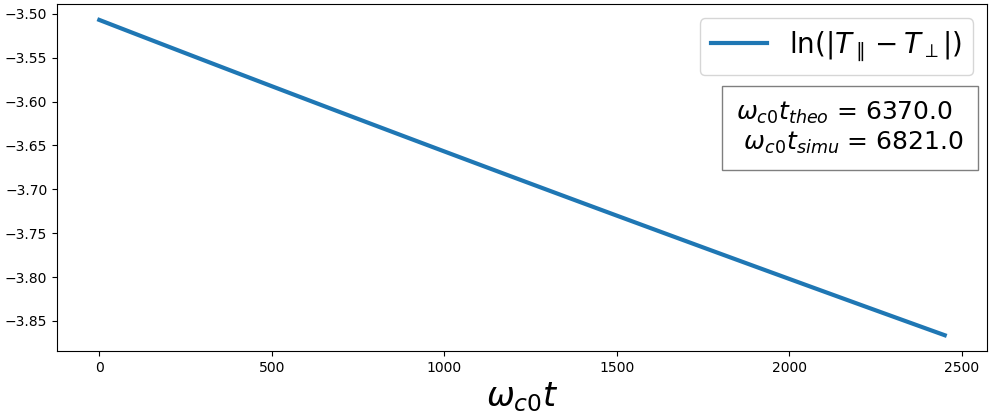
\includegraphics[scale=0.8]{Figures/isotropisation.PNG}
\label{fig: isotropisation}
\end{figure}


\subsection{Test with two species}

The theoretical exchange rates of parallel momentum and energy between two Maxwellians are respectively
\[
R_{\parallel,Mab}=-n_{a}m_{a}\nu_{ab}\left(V_{\parallel a}-V_{\parallel b}\right)
\]


\[
Q_{M,ab}=-3\frac{n_{a}m_{a}}{m_{a}+m_{b}}\nu_{ab}\left(T_{a}-T_{b}\right)
\]


It is then easy to show that 
\[
\frac{d\ln\left(V_{\parallel a}-V_{\parallel b}\right)}{dt}=-\left(\nu_{ab}+\nu_{ba}\right)
\]


\[
\frac{d\ln\left(T_{a}-T_{b}\right)}{dt}=-2\frac{m_{a}\nu_{ab}+m_{b}\nu_{ba}}{m_{a}+m_{b}}
\]


These two relations have been checked using proton and deuterium for the two species. The result for the simulation with different velocities is shown in fig.\ref{fig:Relaxation-Vpar-two-species}. The result for the simulation with different temperatures is shown in fig.\ref{fig:Relaxation-T-two-species}. The agreement is of the order of one percent in both cases.

\begin{figure}[H]
\caption{Relaxation of the parallel velocities of the two species \label{fig:Relaxation-Vpar-two-species}}
\centering{}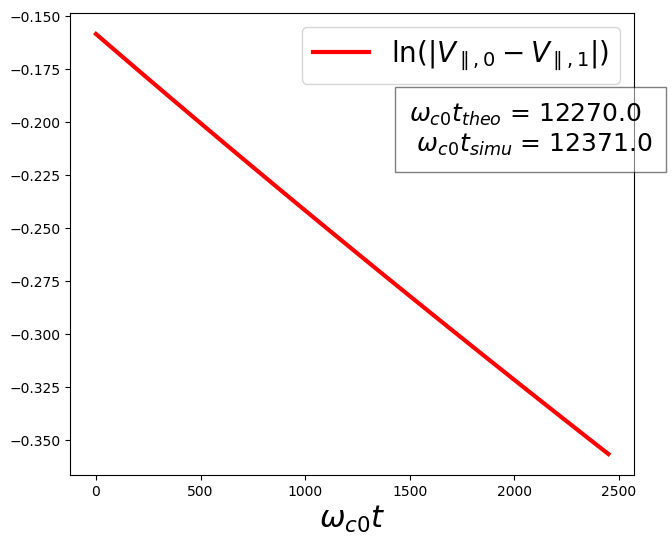
\includegraphics[scale=0.8]{Figures/2_species_velocities.PNG}
\end{figure}


\begin{figure}[H]
\caption{Relaxation of the temperatures of the two species\label{fig:Relaxation-T-two-species}}
\centering{}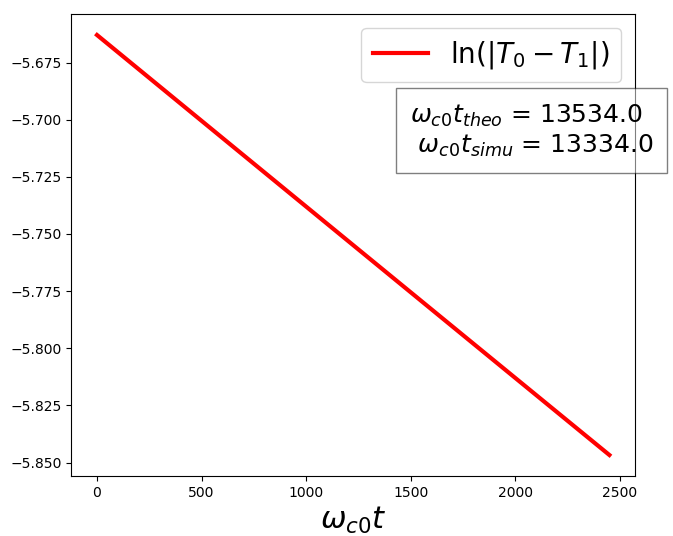
\includegraphics[scale=0.8]{Figures/2_species_temperature.PNG}
\end{figure}

\begin{thebibliography}{1}
    \bibitem{Donnel_CPC_2019} P. Donnel \emph{et al.}, Computer Physics Communications (2019), "A multi-species collisional operator for full-F global gyrokinetics codes: Numerical aspects and verification with the GYSELA code"
\end{thebibliography}



\end{document}
